% Options for packages loaded elsewhere
\PassOptionsToPackage{unicode}{hyperref}
\PassOptionsToPackage{hyphens}{url}
%
\documentclass[
]{book}
\usepackage{lmodern}
\usepackage{amssymb,amsmath}
\usepackage{ifxetex,ifluatex}
\ifnum 0\ifxetex 1\fi\ifluatex 1\fi=0 % if pdftex
  \usepackage[T1]{fontenc}
  \usepackage[utf8]{inputenc}
  \usepackage{textcomp} % provide euro and other symbols
\else % if luatex or xetex
  \usepackage{unicode-math}
  \defaultfontfeatures{Scale=MatchLowercase}
  \defaultfontfeatures[\rmfamily]{Ligatures=TeX,Scale=1}
\fi
% Use upquote if available, for straight quotes in verbatim environments
\IfFileExists{upquote.sty}{\usepackage{upquote}}{}
\IfFileExists{microtype.sty}{% use microtype if available
  \usepackage[]{microtype}
  \UseMicrotypeSet[protrusion]{basicmath} % disable protrusion for tt fonts
}{}
\makeatletter
\@ifundefined{KOMAClassName}{% if non-KOMA class
  \IfFileExists{parskip.sty}{%
    \usepackage{parskip}
  }{% else
    \setlength{\parindent}{0pt}
    \setlength{\parskip}{6pt plus 2pt minus 1pt}}
}{% if KOMA class
  \KOMAoptions{parskip=half}}
\makeatother
\usepackage{xcolor}
\IfFileExists{xurl.sty}{\usepackage{xurl}}{} % add URL line breaks if available
\IfFileExists{bookmark.sty}{\usepackage{bookmark}}{\usepackage{hyperref}}
\hypersetup{
  pdftitle={Python for social and experimental psychology},
  pdfauthor={Alexander Pastukhov},
  hidelinks,
  pdfcreator={LaTeX via pandoc}}
\urlstyle{same} % disable monospaced font for URLs
\usepackage{longtable,booktabs}
% Correct order of tables after \paragraph or \subparagraph
\usepackage{etoolbox}
\makeatletter
\patchcmd\longtable{\par}{\if@noskipsec\mbox{}\fi\par}{}{}
\makeatother
% Allow footnotes in longtable head/foot
\IfFileExists{footnotehyper.sty}{\usepackage{footnotehyper}}{\usepackage{footnote}}
\makesavenoteenv{longtable}
\usepackage{graphicx}
\makeatletter
\def\maxwidth{\ifdim\Gin@nat@width>\linewidth\linewidth\else\Gin@nat@width\fi}
\def\maxheight{\ifdim\Gin@nat@height>\textheight\textheight\else\Gin@nat@height\fi}
\makeatother
% Scale images if necessary, so that they will not overflow the page
% margins by default, and it is still possible to overwrite the defaults
% using explicit options in \includegraphics[width, height, ...]{}
\setkeys{Gin}{width=\maxwidth,height=\maxheight,keepaspectratio}
% Set default figure placement to htbp
\makeatletter
\def\fps@figure{htbp}
\makeatother
\setlength{\emergencystretch}{3em} % prevent overfull lines
\providecommand{\tightlist}{%
  \setlength{\itemsep}{0pt}\setlength{\parskip}{0pt}}
\setcounter{secnumdepth}{5}
\usepackage{booktabs}
\usepackage[]{natbib}
\bibliographystyle{apalike}

\title{Python for social and experimental psychology}
\author{Alexander Pastukhov}
\date{2020-10-23}

\begin{document}
\maketitle

{
\setcounter{tocdepth}{1}
\tableofcontents
}
\hypertarget{introduction}{%
\chapter*{Introduction}\label{introduction}}
\addcontentsline{toc}{chapter}{Introduction}

\hypertarget{about-the-seminar}{%
\section*{About the seminar}\label{about-the-seminar}}
\addcontentsline{toc}{section}{About the seminar}

This is a material for \emph{Python for social and experimental psychology} seminar. Each chapter covers a single seminar, introducing necessary ideas and is accompanied by a notebook with exercises, which you need to complete and submit. The material assumes no foreknowledge of Python or programming from the reader. Its purpose is to gradually build up your knowledge and allow you to create more and more complex games. Yes, games! Of course, the real research is about performing experiments but there is little difference between the two. The basic ingredients are the same and, arguably, experiments are just boring games. And, be assured, if you can program a game, you certainly can program an experiment.

We will start with simple \emph{Guess a Number} text-only game with first you and then the computer doing the guessing. Next, we will implement a classic \emph{Hunt the Wumpus} text adventure game that will require use of more complex structures. Once we master the basics, we will up the ante by making a video game with graphics and sounds using \href{https://psychopy.org/}{PsychoPy} library to code a classic \emph{Memory Game}. Finally, we will create a more dynamic game by making a clone of a \emph{Flappy Bird}.

Remember that throughout the seminar you can and should(!) always ask me whenever something is unclear, you do not understand a concept or logic behind certain code. Do not hesitate to write me in the team or (better) directly to me in the chat (in the latter case, the notifications are harder miss and we don't spam others with our conversation).
As a final assignment, you will need to program a (currently mysterious) video game, which will only require the material covered by the seminar. Please inform me, If you require a grade, as then I will create a more specific description for you to have a clear understanding of how the program will be graded.

\hypertarget{why-python}{%
\section*{Why Python?}\label{why-python}}
\addcontentsline{toc}{section}{Why Python?}

The ultimate goal of this seminar is to teach you how to create an experiment for psychology research. There are many ways to achieve this end. You can use drag-and-drop systems either commercial like \href{https://www.neurobs.com/}{Presentation}, \href{https://www.sr-research.com/experiment-builder/}{Experiment Builder} or free like \href{https://psychopy.org/builder}{PsychoPy Bulder interface}. They have a much shallower learning curve, so you can start creating and running your experiments faster. However, the simplicity of their use has the price: They are fairly limited in which stimuli you can use and how you can control the presentation schedule, feedback, etc. Typically, they allow you to extend them by programming the desired behavior but you do need to know how to program to do this. Thus, I think that while these systems, in particular \href{https://psychopy.org/}{PsychoPy}, are great tools to quickly bang a simple experiment together, they are most useful if you understand how they create the code and how you would program it yourself. Then, you will not fill being limited by the software, as you know you can program something the default drag-and-drop won't allow, but you can always opt in, if drag-and-drop is sufficient but faster. At the end, it is about having options and creative freedom to program an experiment that will answer your research question, not an experiment that your software allows you to program.

We will learn programming in Python, which is a great language that combines simple and clear syntax with power and ability to tackle almost any problem. The advantage of learning Python, as compared to say Matlab, which is commonly used in neuroscience, is that it allows you do almost anything. In this seminar, we will concentrate on desktop experiments but you can use it for online experiments (\href{https://otree.readthedocs.io/en/latest/}{oTree}), scientific programming (\href{https://numpy.org/}{NumPy} and \href{https://www.scipy.org/}{SciPy}), data analysis (\href{https://pandas.pydata.org/}{pandas}), machine learning (\href{https://keras.io/}{keras}), website programming (\href{https://www.djangoproject.com/}{django}), computer vision (\href{https://opencv.org/}{OpenCV}), etc. Thus, learning Python will give you one of the most versitile programming tools that you can use for all stages of your research or work. And, Python is free, so you do not need to worry whether you or your future employer will be able to afford the license fees (a very real problem, if you use Matlab).

\hypertarget{getting-started}{%
\chapter*{Getting Started}\label{getting-started}}
\addcontentsline{toc}{chapter}{Getting Started}

\hypertarget{install-anaconda}{%
\section*{Installing Anaconda environment}\label{install-anaconda}}
\addcontentsline{toc}{section}{Installing Anaconda environment}

First, install \href{https://www.anaconda.com}{Anaconda}, a Python distribution that includes many packages and tools out-of-the-box, makes it easy to install new packages and keep them updated. Follow this \href{https://www.anaconda.com/products/individual}{link} and download the installer suitable for your platform. You can pick either 32- or 64-bit version but I would recommend the latter, so that we all have maximally similar setup (it won't really make a difference in practice, though). Follow the installer instructions and use defaults, unless you have reasons to modify them (e.g.~folder location, as the drive for the default choice may have limited available space, as in my case).

After installation you will have a new \emph{Anaconda3 (64-bit)} folder that contains links to programs.

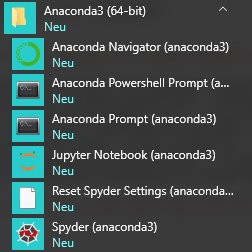
\includegraphics[width=3.5in]{images/anaconda-shortcuts}

You can use \emph{Anaconda Navigator} that allows you to choose a specific programming environment, including \href{https://jupyter.org/}{Jupyter Notebook} that we will use (not JupyterLab, it more versatile but we want to keep things simple at the beginning!). Alternatively, you can start \emph{Jupyter Notebook} directly from the start menu. Please read the \href{https://jupyter-notebook.readthedocs.io/en/stable/examples/Notebook/examples_index.html}{online documentation} to familiarize yourself with Jupyter Notebook basic interface, e.g.~how to create a new cell, run it, etc.

\hypertarget{install-vs-code}{%
\section*{Installing Visual Studio Code}\label{install-vs-code}}
\addcontentsline{toc}{section}{Installing Visual Studio Code}

\href{https://code.visualstudio.com/}{Visual Studio Code} is a lightweight free open-source editor with strong support for Python. We will start use it in earnest, once our programs grow to be sufficiently long and complex. At the early stages, we will mostly use Jupyter notebooks and I would recommend using Jupyter notebooks using the default browser-based editor you installed as part of \protect\hyperlink{install-anaconda}{Anaconda}. However, you can also work with Jupyter notebooks in VS Code \href{https://code.visualstudio.com/docs/python/jupyter-support}{directly}.

As in case of \protect\hyperlink{install-anaconda}{Anaconda}, download the installer for your platform and follow the instructions. Start VS Code and open any Python file, for example \href{other/empty.py}{this one} (use \texttt{Alt+click} to download it, ignore warnings, it is has only comments, so cannot harm you). When you open Python file for the first time, VS Code will suggest to install a Python extension. Do just that andinstall a linter as well when VS Code suggests that (\href{https://code.visualstudio.com/docs/python/linting}{linting} highlights syntactical and stylistic problems in your code, making it easier to write consistent clear code).

Once the Python extension is activated, you will see which Python interpreter is used (you can have more than one or you may use have multiple \href{https://docs.python.org/3/tutorial/venv.html}{virtual environments}).


\includegraphics[width=6.96in]{images/vscode-python-interpreter}
If the selected environment is the wrong one or you are simply not sure, click on it and it will open a drop-down list with all interpreters and environments you have. Consult VS Code \href{https://code.visualstudio.com/docs/python/environments}{online documentation} on environments, if you need to change/add/delete environment (the exact settings may change, so looking at constantly updated online documentation is wiser than copying it here, so it would be outdated quite soon).

\hypertarget{install-psychopy}{%
\section*{Installing PsychoPy}\label{install-psychopy}}
\addcontentsline{toc}{section}{Installing PsychoPy}

This step can wait until the first \protect\hyperlink{memory-game-01}{Memory Game} seminar.

Download and install \href{https://www.psychopy.org/download.html}{Standalone PsychoPy} version. You can install PsychoPy as a conda package or via pip but using it as a standalone would ensure that you have all necessary additional libraries and a builder interface for the future use. We will use PsychoPy's python environment in \protect\hyperlink{install-vs-code}{VS Code}.

\end{document}
